\item As per given figure, a weightless pulley P is attached on a double inclined frictional surfaces. The tension in the string (massless) will be (if \(g = 10 \, \text{m/s}^2\))
    \begin{center}
        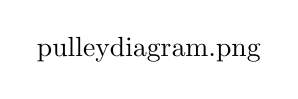
\begin{tikzpicture}
            \node at (0, 0) {{pulleydiagram.png}};
        \end{tikzpicture}
    \end{center}
    \begin{tasks}(2)
        \task \( 4\left(\sqrt{3} - 1\right) \text{N} \)
        \task \( 4\left(\sqrt{3} + 1\right) \text{N} \)
        \task (C) \(4\sqrt{3} - 1\text{N} \)
        \task \( (4\sqrt{3} + 1\text{N} \)
    \end{tasks}